\section{Method}
\label{sec:method}

Phantom recovers two geometry layers from images of a scene with transparent objects: for every view, the visible front surface of each object and the scene seen through it.
Instead of training a new geometry network, we train two light image front-ends that translate the input into images a frozen, off-the-shelf geometry backbone already handles well, and then merge the backbone's two predictions (\cref{fig:method}).

\subsection{Problem Formulation}
\label{sec:formulation}

Given $N \ge 1$ views of the same scene, we denote the $i$-th view with known camera intrinsics $K_i$ as
\[
  I_i \in [0,1]^{H \times W \times 3}, \qquad i=1,\ldots,N.
\]
For each view, TransDINO~\cite{ghost} predicts the transparent-object mask
\[
  \hat M_i = \operatorname{TransDINO}(I_i) \in \{0,1\}^{H \times W}.
\]
Inside the mask, a pixel observes two surfaces at once: the front surface of the transparent object and, refracted and attenuated, the scene behind it.
A geometry backbone trained on opaque scenes predicts neither reliably and typically returns a mixture of the two.
We therefore assign each layer its own image:
\begin{equation}
  \begin{aligned}
  \{\hat B_i\}_{i=1}^{N} &= \mathcal{F}_{bg}\big(\{I_i, \hat M_i, P_i\}_{i=1}^{N}\big), \\
  \hat O_i &= \mathcal{F}_{sf}(I_i, \hat M_i),
  \end{aligned}
  \label{eq:frontends}
\end{equation}
where $\hat B_i$ is view $i$ with the transparent objects removed (objects behind or inside them are kept), $\hat O_i$ is the same view with every transparent object rendered as an opaque diffuse surface, and $P_i$ is a LaMa inpainting~\cite{lama} of $I_i$ inside $\hat M_i$.
$\mathcal{F}_{bg}$ receives all views of the scene and can exchange information between them; $\mathcal{F}_{sf}$ handles each view on its own.
Everything after the front-ends is done per view, so from here on we drop the view index.
A frozen geometry backbone $\mathcal{G}$ predicts a depth map for each image, which we back-project with $K$ (denoted $\Pi_K^{-1}$) into the background cloud $X_{bg}$ and the candidate surface cloud $X_{sf}$:
\begin{equation}
  X_{bg} = \Pi_K^{-1}\big(\mathcal{G}(\hat B)\big), \qquad X_{sf} = \Pi_K^{-1}\big(\mathcal{G}(\hat O)\big).
  \label{eq:backbone}
\end{equation}
$\mathcal{G}$ is any single-image or feed-forward geometry model; we use VGGT~\cite{vggt}, $\pi^3$~\cite{pi3}, Depth Anything V2 Metric~\cite{dav2}, Depth Anything 3~\cite{da3}, MoGe-2~\cite{moge2} and MoGe-3~\cite{moge3} without fine-tuning.
The front-ends are trained once and reused for every backbone.

\subsection{Front-End Architecture}
\label{sec:architecture}

$\mathcal{F}_{bg}$ and $\mathcal{F}_{sf}$ use the same encoders, decoder and output head (\cref{fig:method}) but are trained separately and keep separate weights.
Only $\mathcal{F}_{bg}$ has the prior input and the cross-view attention.
Both work at $294 \times 518$ and edit only the masked region.

% TODO(data swap): state the DINOv3 variant actually used. The code supports ViT-S/16 (layers 3/6/9/12)
% and ViT-L/16 (layers 6/12/18/24); the text below holds for both.
\paragraph{Encoders.}
A frozen DINOv3 ViT~\cite{dinov3} provides semantic context on a $21 \times 37$ token grid.
The mask enters through a zero-initialized patch convolution added to the tokens, so training starts from the pretrained features.
Tokens from four evenly spaced layers are projected, concatenated and fused by two $3{\times}3$ convolutions (\emph{Fusion} in \cref{fig:method}).
Because these features have only $1/16$ of the image resolution, a small trainable CNN computes detail features at $1/2$, $1/4$ and $1/8$ resolution from $I$, $\hat M$ and, for $\mathcal{F}_{bg}$, $P$.

% TODO(data swap): 4 attention pairs, 6 heads and 4 training views are the settings of the existing
% multi-view run (bg_mv4); confirm them for the final DINOv3 model.
\paragraph{Cross-view attention.}
In $\mathcal{F}_{bg}$, the fused features of the $N$ views pass through four pairs of attention blocks before decoding; each pair applies self-attention within each view and then across all views, following VGGT~\cite{vggt}.
Zero-initialized residual scales make the module start as the identity.
It uses no camera poses, depth or epipolar constraints; $\mathcal{F}_{sf}$ has no attention layers.

\paragraph{Decoder and output head.}
A convolutional decoder (\emph{RGB decoder} in \cref{fig:method}) upsamples the features in three stages, concatenating the detail features of matching resolution at each stage, and at full resolution concatenates the input image, the mask and (for $\mathcal{F}_{bg}$) the prior.
A single $3{\times}3$ convolution produces all outputs.
The main output is an RGB residual $r$ applied in logit space,
\begin{equation}
  C = \sigma\big(r + \operatorname{logit}(\operatorname{clip}(I, 0.02, 0.98))\big),
  \label{eq:residual}
\end{equation}
so that a zero residual reproduces the (clipped) input.
$\mathcal{F}_{bg}$ also outputs two fusion logits $(\ell_c, \ell_p)$ that select, per pixel, between its own prediction $C$ and the LaMa prior $P$ (\emph{Mix} in \cref{fig:method}).

\paragraph{Masked composition.}
Both front-ends paste their prediction into the input inside the mask (\emph{Mask} in \cref{fig:method}; for $\mathcal{F}_{bg}$ this step is part of \emph{Mix}).
To avoid seams at the mask boundary, we feather the mask, $\tilde M = \operatorname{AvgPool}_5(\operatorname{MaxPool}_5(\hat M))$, and compose
\begin{align}
  \hat B &= \tilde M \odot (w_c C_{bg} + w_p P) + (1 - \tilde M) \odot I, \label{eq:compose-bg} \\
  \hat O &= \tilde M \odot C_{sf} + (1 - \tilde M) \odot I, \label{eq:compose-sf}
\end{align}
where $(w_c, w_p) = \operatorname{softmax}(\ell_c, \ell_p)$ per pixel, and $C_{bg}$ and $C_{sf}$ are the outputs of \cref{eq:residual} for the two front-ends.

\subsection{Training Objective}
\label{sec:training}

Each front-end is trained on synthetic data (\cref{sec:data}) against its own target image $Y^*$: the rendered background $B^*$ for $\mathcal{F}_{bg}$ and the rendered opaque image $O^*$ for $\mathcal{F}_{sf}$.
Let $\hat Y$ be the front-end output, $M$ the ground-truth mask, $R$ the mask dilated by 3\,px, and $T \subseteq M$ the through region, where the background seen through the glass is another object rather than the support surface.
The loss is
\begin{equation}
  \begin{split}
  \mathcal{L} = {}&\mathcal{L}_{1} + \lambda_{p}\mathcal{L}_{\mathrm{LPIPS}} + \lambda_{o}\mathcal{L}_{\mathrm{out}} \\
  &+ \lambda_{f}\mathcal{L}_{\mathrm{flow}} + \lambda_{v}\mathcal{L}_{\mathrm{vis}} + \lambda_{g}\mathcal{L}_{\mathrm{geo}}.
  \end{split}
  \label{eq:loss}
\end{equation}

\paragraph{Image terms.}
$\mathcal{L}_{1}$ is the per-pixel L1 error weighted by $\omega = R \odot (1 + \lambda_t T)$ and normalized by $\sum \omega$.
For $\mathcal{F}_{bg}$ we set $\lambda_t = 2$, so through pixels, which carry the information that inpainting cannot provide, count three times; for $\mathcal{F}_{sf}$, $\lambda_t = 0$.
$\mathcal{L}_{\mathrm{LPIPS}}$ is the VGG LPIPS distance~\cite{lpips} between $Y^*$ and an image that equals $\hat Y$ inside $R$ and $Y^*$ elsewhere, divided by the area fraction of $R$.
$\mathcal{L}_{\mathrm{out}}$ is the mean L1 error outside $R$ and keeps the feathered band close to the input.

\paragraph{Auxiliary refraction terms.}
Both front-ends also predict a backward refraction flow, which maps each masked pixel to the background pixel seen through the glass, and a logit for whether that point is visible; neither is used to form the output image.
$\mathcal{L}_{\mathrm{flow}}$ is the L1 error of this flow where the ground truth is defined and visible, and $\mathcal{L}_{\mathrm{vis}}$ is the binary cross-entropy of the visibility logit inside $R$.

\paragraph{Geometry-aware term.}
An image can be close to $Y^*$ in color and still lead a backbone to a different depth.
We therefore pass both $\hat Y$ and $Y^*$ through a frozen depth network $D$ (Depth Anything V2 Metric, ViT-S~\cite{dav2}) and penalize the mean-centered log-depth difference inside $R$:
\begin{equation}
  \begin{split}
  \Delta &= \log D(\hat Y) - \log D(Y^*), \\
  \mathcal{L}_{\mathrm{geo}} & = \frac{1}{|R|}\sum_{x \in R} \Big|\Delta(x) - \bar\Delta_R\Big|,
  \end{split}
  \label{eq:geo}
\end{equation}
where $\bar\Delta_R$ is the mean of $\Delta$ over $R$.
Subtracting the mean makes the term invariant to a global depth scale, and because it compares two predictions of $D$, it needs no ground-truth depth.
$D$ is smaller than, and separate from, the backbones used at test time.

\paragraph{Settings.}
We use $\lambda_p = \lambda_o = 0.2$, $\lambda_f = 0.05$, $\lambda_v = 0.1$ and $\lambda_g = 0.5$ for both front-ends.
The input mask is the ground-truth mask with random morphological perturbations, so the front-ends learn to handle imperfect masks.
% TODO(data swap): batch size and views per scene of the final multi-view F_bg run.
Each front-end is trained for 40k iterations with AdamW~\cite{adamw}, and $\mathcal{F}_{bg}$ on groups of four views of the same scene.
Only the mask adapter, detail CNN, cross-view attention, decoder and head are trained.
Augmentations and optimizer settings are given in the supplement.

\begin{figure}[t]
  \centering
  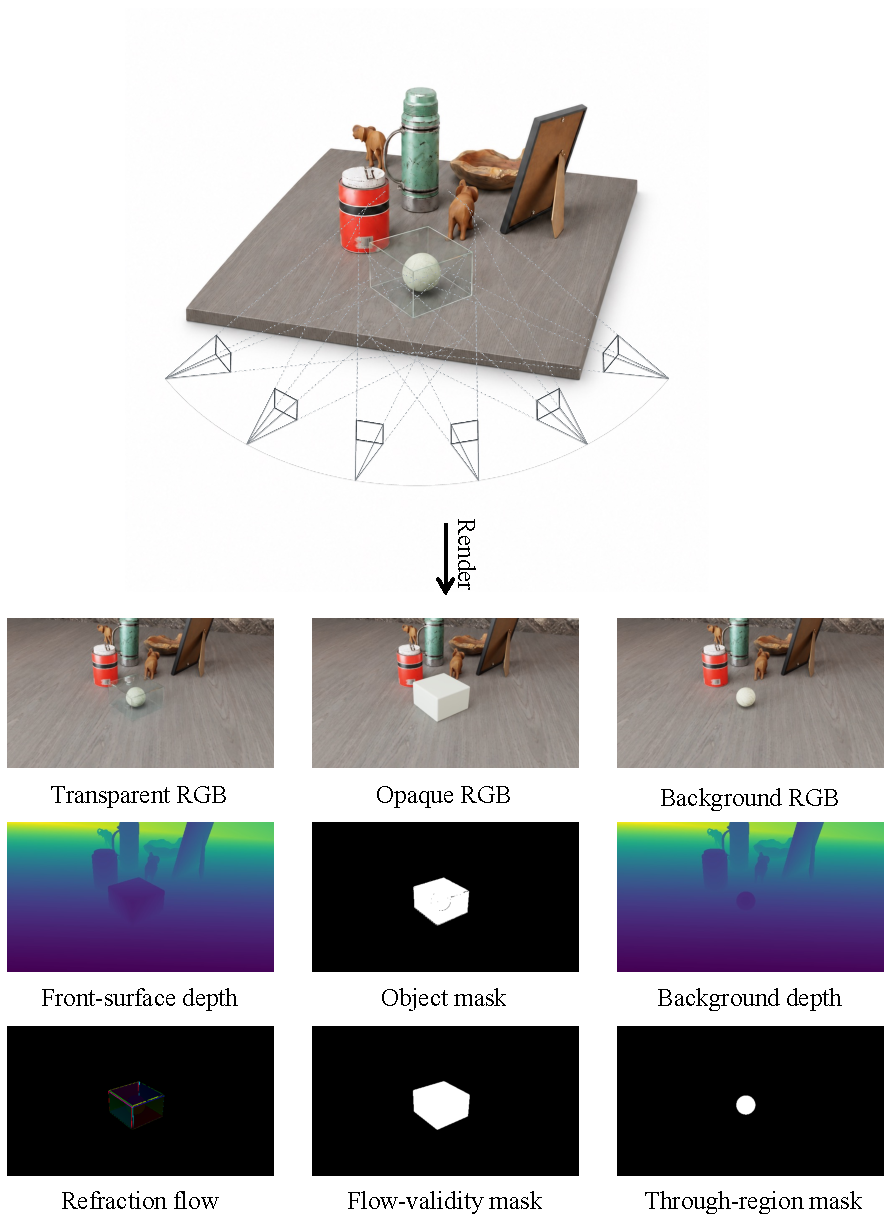
\includegraphics[width=\columnwidth]{fig/dataset/output/dataset_slide4.pdf}
  \caption{\textbf{Synthetic two-layer data.}
  Top: multi-view rendering setup.
  Bottom: per-view inputs and targets (RGB, opaque and background images, both depths, mask, refraction flow, flow validity and through region).}
  \label{fig:synthetic-data}
\end{figure}

\subsection{Layered Geometry Fusion}
\label{sec:fusion}

Because $\mathcal{G}$ runs on $\hat B$ and $\hat O$ separately, its two predictions are related by an unknown similarity transform, and backbones that predict only relative depth add a free scale.
We estimate this transform from the region where the two images agree.

\paragraph{Correspondences.}
Let $\Omega$ be the pixels outside $\hat M$ dilated by 7\,px at which both predictions are valid.
Outside the mask, $\hat B$ and $\hat O$ show the same scene, so for $x \in \Omega$ the points $X_{sf}(x)$ and $X_{bg}(x)$ should coincide.
These same-pixel pairs serve as correspondences and require no feature matching.
We randomly hold out 20\% of $\Omega$ for diagnostics and sample at most 8,000 of the remaining pixels for fitting.

\paragraph{Robust Sim(3).}
We seek $(s, \mathbf{R}, \mathbf{t})$ that minimize
\begin{equation}
  \sum_{x \in \Omega_{\mathrm{in}}} \big\| s\mathbf{R}\,X_{sf}(x) + \mathbf{t} - X_{bg}(x) \big\|^2 ,
  \label{eq:sim3}
\end{equation}
where $\Omega_{\mathrm{in}}$ is the set of inliers.
The predictions near depth discontinuities and in the feathered band can disagree strongly, so a plain least-squares fit over all of $\Omega$ is unreliable.
We run 250 RANSAC~\cite{ransac} iterations, each fitting a closed-form Umeyama~\cite{umeyama} solution to 6 random pairs and counting pairs with residual below $\tau = 0.025\,\mathrm{med}_{x}\|X_{bg}(x)\|$.
The hypothesis with the most inliers is refined by refitting on its inliers five times.

\paragraph{Layered point cloud.}
The final representation keeps every background point and adds the aligned surface points inside the mask:
\begin{equation}
  \mathcal{P} = \big\{X_{bg}(x)\big\}_{x} \;\cup\; \big\{s\mathbf{R}\,X_{sf}(x) + \mathbf{t} \;\big|\; \hat M(x) = 1\big\}.
  \label{eq:fusion}
\end{equation}
Each point carries a layer label: background outside the mask (0), background seen through the transparent object (1), and transparent front surface (2).
Inside the mask, the scene therefore has two depths per pixel, which a single prediction from $\mathcal{G}$ cannot represent.
Since $X_{bg}$ is the anchor, it fixes the scale and pose of the whole layered scene; it inherits any scale ambiguity of $\mathcal{G}$.

\subsection{Synthetic Two-Layer Data}
\label{sec:data}

Real images with ground truth for both the front surface and the scene behind it are not available, so we render training data with Blender Cycles (\cref{fig:synthetic-data}).
Each scene places transparent objects (cups, glasses, bottles, bowls, boxes, solid glass and thin films) on a textured table under indoor HDRI lighting, with scanned opaque props behind them and, in some containers, inside them, and is viewed by several cameras.
For every view we render the input $I$, the background target $B^*$ with all transparent objects hidden, the opaque target $O^*$ with every transparent material replaced by an opaque diffuse one, the masks $M$ and $T$, the depth of both layers, and the refraction flow.
Because all targets share the camera and lighting of $I$, the supervision isolates the effect of the transparent object.
We render three sets: \emph{Oblique} (4 oblique cameras per scene, 4--8 props), \emph{Clutter} (6--11 props, half of the scenes seen from nearly above as by a robot-arm camera, opaque labels and thicker glass) and \emph{Wide} (Clutter scenes seen by 6 cameras covering about 125\textdegree).
Rendering parameters are given in the supplement.
